\section*{Introduction}
	\begin{frame}
		\frametitle{Introduction}
		\begin{itemize}
			\item<1-> Advancements in AI/ML for IoT and TinyML
			\item<2-> Need for energy efficiency
			\item<3-> Hybrid precision approach
			\item<4-> Design challenges
			\item<5-> Approximate computing and quantization
			\item<6-> Quality, interoperability, and compatibility
		\end{itemize}
	\end{frame}
	
	\section*{Goal and Objectives}
	\begin{frame}
		\frametitle{Goal and Objectives}
		\begin{itemize}
			\item<1-> Goal:
			To develop advanced methodologies for energy-efficient neural network accelerators with custom floating-point (FP) computation in low-power and resource constrained devices.
			\item<2-> Objectives:
			\begin{itemize}
				\item<3-> Optimal custom FP number representation
				\item<4-> Energy-efficient design strategies and custom FP arithmetic units
				\item<5-> Precision and quantization impact analysis
				\item<6-> Hardware performance evaluation and bench marking
				\item<7-> Practical application
				\item<8-> Future research
			\end{itemize}
		\end{itemize}
	\end{frame}

	\begin{frame}
	\frametitle{Outline}
	\tableofcontents % This command automatically creates a table of contents based on the sections and subsections
	\end{frame}
	
	\section{State-of-the-Art}
	\tableofcontents[currentsection]
	
	\begin{frame}{High-Performance FPGA-Based CNN Accelerator With Block-Floating-Point Arithmetic}
		\centering
		\begin{figure}
			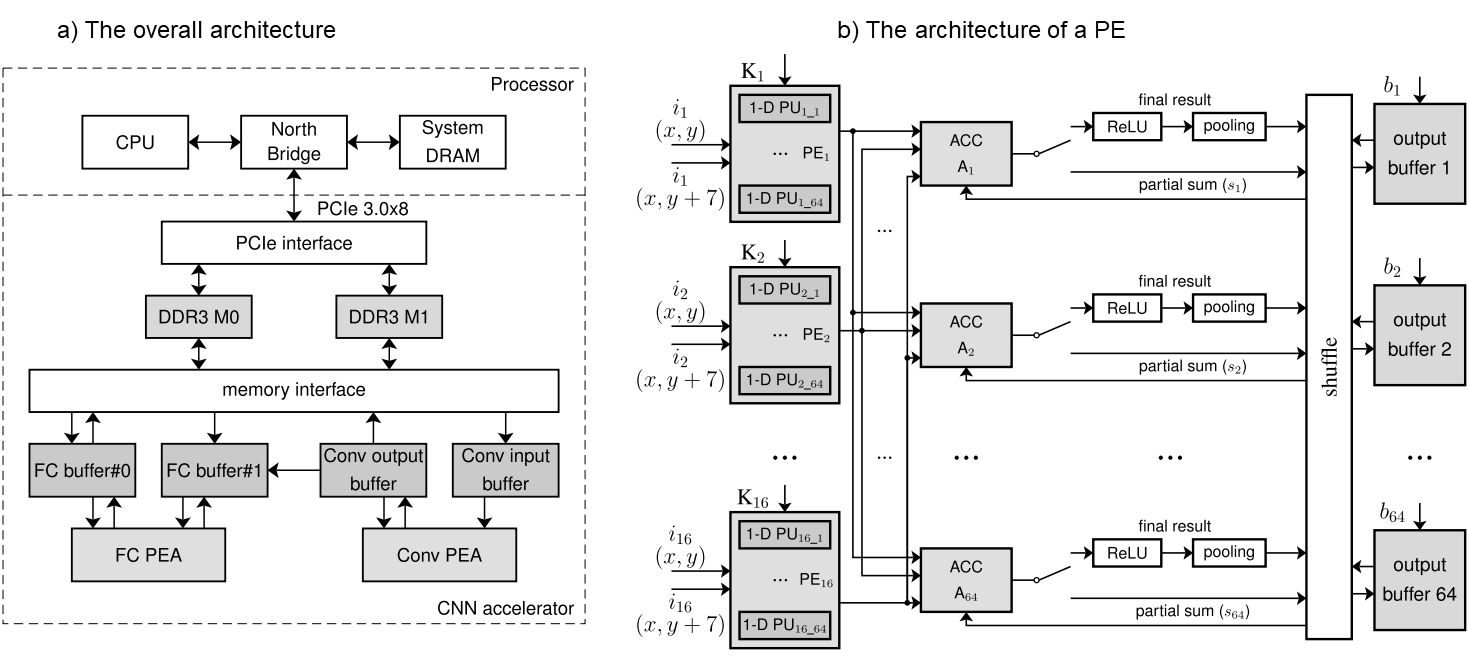
\includegraphics[width=\textwidth]{../figures/3_g.png}
			\caption{(a) System architecture. (b) Processing element array.}
		\end{figure}
	\end{frame}
	
	\begin{frame}{A 200MHZ 202.4GFLOPS@10.8W VGG16 Accelerator in Xilinx VX690T}
		\centering
		\begin{figure}
			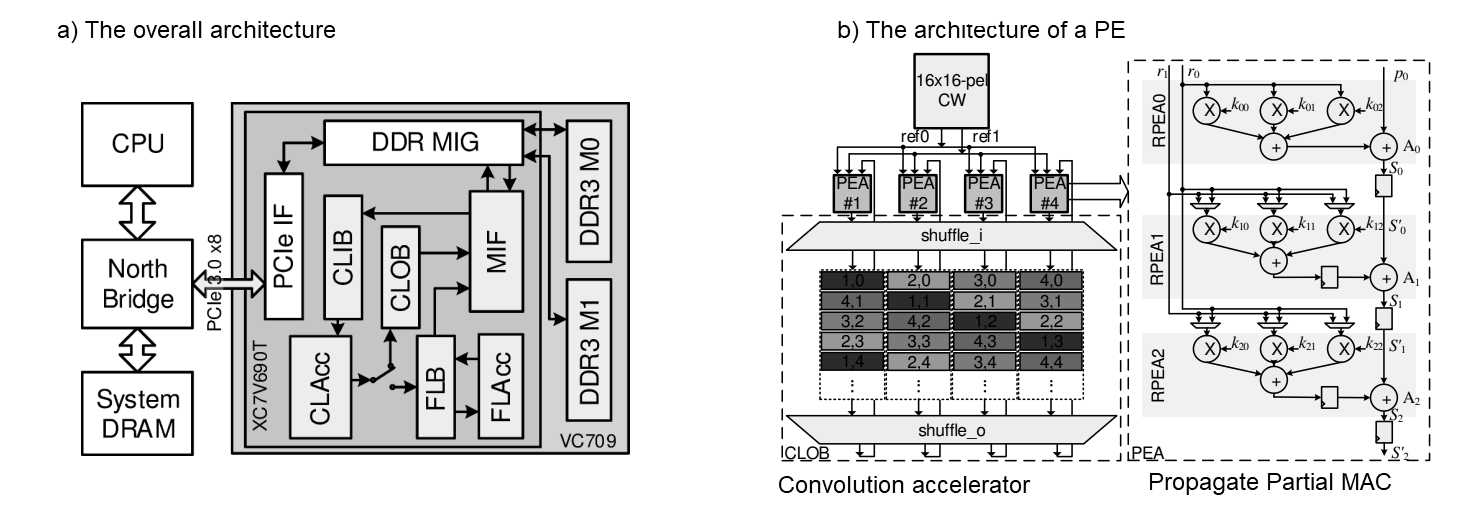
\includegraphics[width=\textwidth]{../figures/1_g.png}
			\caption{(a) System architecture. (b) Convolution accelerator.}
		\end{figure}
	\end{frame}
	
	\begin{frame}{Low-precision Floating-point Arithmetic for High-performance FPGA-based CNN Acceleration}
		\centering
		\begin{figure}
			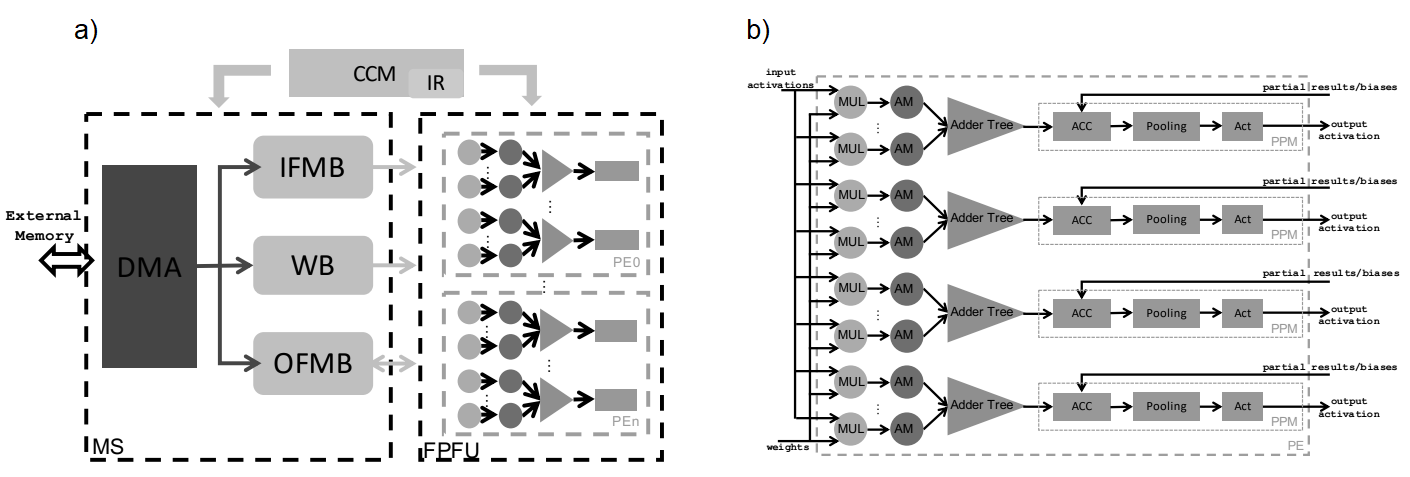
\includegraphics[width=\textwidth]{../figures/2_g.png}
			\caption{(a) System architecture. (b) Processing element.}
		\end{figure}
	\end{frame}

	\begin{frame}{CNN Hardware Acceleration on a Low-Power and Low-Cost APSoC}
	\centering
	\begin{figure}
		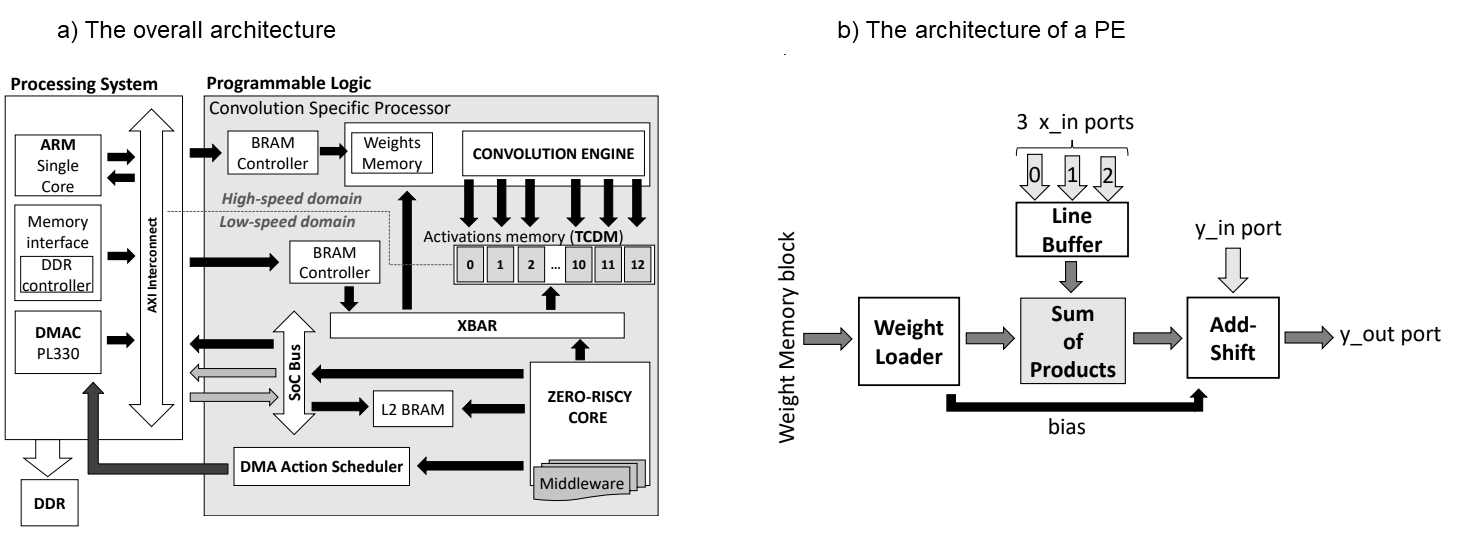
\includegraphics[width=\textwidth]{../figures/4_g.png}
		\caption{(a) System architecture. (b) Convolution engine.}
	\end{figure}
	\end{frame}